%% Template for MLP Coursework 2 / 6 November 2017 

%% Based on  LaTeX template for ICML 2017 - example_paper.tex at 
%%  https://2017.icml.cc/Conferences/2017/StyleAuthorInstructions

\documentclass{article}
\usepackage[T1]{fontenc}
\usepackage{amssymb,amsmath}
\usepackage{txfonts}
\usepackage{microtype}

% For figures
\usepackage{graphicx}
\usepackage{subfigure} 

% For citations
\usepackage{natbib}

% For algorithms
\usepackage{algorithm}
\usepackage{algorithmic}

% the hyperref package is used to produce hyperlinks in the
% resulting PDF.  If this breaks your system, please commend out the
% following usepackage line and replace \usepackage{mlp2017} with
% \usepackage[nohyperref]{mlp2017} below.
\usepackage{hyperref}
\usepackage{url}
\urlstyle{same}

% Packages hyperref and algorithmic misbehave sometimes.  We can fix
% this with the following command.
\newcommand{\theHalgorithm}{\arabic{algorithm}}


% Set up MLP coursework style (based on ICML style)
\usepackage{mlp2018}
\mlptitlerunning{MLP Coursework 1 (\studentNumber)}
\bibliographystyle{icml2017}


\DeclareMathOperator{\softmax}{softmax}
\DeclareMathOperator{\sigmoid}{sigmoid}
\DeclareMathOperator{\sgn}{sgn}
\DeclareMathOperator{\relu}{relu}
\DeclareMathOperator{\lrelu}{lrelu}
\DeclareMathOperator{\elu}{elu}
\DeclareMathOperator{\selu}{selu}
\DeclareMathOperator{\maxout}{maxout}


%% You probably do not need to change anything above this comment

%% REPLACE this with your student number
\def\studentNumber{s1502810}
\usepackage{multirow}
\usepackage{array}
\usepackage{booktabs}
\usepackage{amsmath}
\usepackage{graphicx}
\usepackage{float} 
\usepackage{subfigure}
\usepackage{upgreek}
\usepackage{leftidx}

\begin{document} 

\twocolumn[
\mlptitle{MLP Coursework 1: Learning Algorithms and Regularization}

\centerline{s1502810}

\vskip 7mm
]

\begin{abstract} 

Optimization has always been an important topic in the field of neural networks. It is precisely because of continuous optimization that neural networks can be applied to various fields in reality. Optimization is also the main content of this report. By comparing various gradient descent algorithms, different optimization methods are found to optimize them.

\end{abstract} 

\section{Introduction}
\label{sec:intro}

Learning rate is a very important hyperparameter of neural network. For its debugging, it can affect the fitting speed and fitting degree of a neural network. A good learning rate can greatly improve the accuracy of neural networks. Similarly, the gradient descent algorithm is also very important for the optimization of the neural network. The quality of the gradient descent algorithm also affects the fitting speed and accuracy of the neural network. So this report will focus on these two aspects. In the first part, we will use SGD to train the neural network. In the second part, we will compare the traditional SGD algorithm with the later improved RMSProp algorithm and Adam algorithm. Part III We will use the scheduler to optimize the choice of learning rate. In the last part we will focus on the ge of the Adam algorithm.The experimental method is mainly to train the best neural network by adjusting the learning rate, and then verify by the test data. This data set is taken from Balanced EMINST, a total of three: training data (100000), valid data (15800), test data (15800).


\section{Baseline systems} 

In this section, in order to get the best performance of stochastic gradient descent (SGD) in 2-5 hidden layers as the baseline, I debugged the learning rate hyperparameter. Firstly I will compare these systems using the valid data set and find the best learning rate.


% Table generated by Excel2LaTeX from sheet 'Sheet1'
\begin{table}[htbp]
  \centering
  \caption{accuracy(valid) for different layers and different learning rate}
    \begin{tabular}{|r|r|r|r|r|}
    \toprule
    \multicolumn{1}{|r|}{\multirow{2}[2]{*}{learning\_rate}} & \multicolumn{1}{r|}{\multirow{2}[2]{*}{2 Hidden}} & \multicolumn{1}{r|}{\multirow{2}[2]{*}{3 Hidden}} & \multicolumn{1}{r|}{\multirow{2}[2]{*}{4 Hidden}} & \multicolumn{1}{r|}{\multirow{2}[2]{*}{5 Hidden}} \\
          &       &       &       &  \\
    \midrule
    \multirow{2}[2]{*}{0.1} & \multirow{2}[2]{*}{8.15E-01} & \multirow{2}[2]{*}{8.15E-01} & \multirow{2}[2]{*}{8.17E-01} & \multirow{2}[2]{*}{8.17E-01} \\
          &       &       &       &  \\
    \midrule
    \multirow{2}[2]{*}{0.05} & \multirow{2}[2]{*}{8.28E-01} & \multirow{2}[2]{*}{8.28E-01} & \multirow{2}[2]{*}{8.27E-01} & \multirow{2}[2]{*}{8.29E-01} \\
          &       &       &       &  \\
    \midrule
    \multirow{2}[2]{*}{0.01} & \multirow{2}[2]{*}{8.35E-01} & \multirow{2}[2]{*}{8.35E-01} & \multirow{2}[2]{*}{8.39E-01} & \multirow{2}[2]{*}{8.32E-01} \\
          &       &       &       &  \\
    \midrule
    \multirow{2}[2]{*}{0.0075} & \multirow{2}[2]{*}{8.30E-01} & \multirow{2}[2]{*}{8.42E-01} & \multirow{2}[2]{*}{8.42E-01} & \multirow{2}[2]{*}{8.32E-01} \\
          &       &       &       &  \\
    \midrule
    \multirow{2}[2]{*}{0.005} & \multirow{2}[2]{*}{8.22E-01} & \multirow{2}[2]{*}{8.22E-01} & \multirow{2}[2]{*}{8.28E-01} & \multirow{2}[2]{*}{8.33E-01} \\
          &       &       &       &  \\
    \bottomrule
    \end{tabular}%
  \label{tab:addlabel}%
\end{table}%




Then I use the test data to compare the accuracy of these best systems.

% Table generated by Excel2LaTeX from sheet 'Sheet2'
\begin{table}[htbp]
  \centering
  \caption{the best learning rate for 2-5 Hidden Layers using test set}
    \begin{tabular}{|c|c|c|}
    \toprule
    \multicolumn{1}{|c|}{\multirow{2}[2]{*}{2 Hidden layers}} & \multirow{2}[2]{*}{1.00E-02} & \multirow{2}[2]{*}{8.23E-01} \\
          &       &  \\
    \midrule
    \multicolumn{1}{|c|}{\multirow{2}[2]{*}{3 Hidden layers}} & \multirow{2}[2]{*}{7.50E-03} & \multirow{2}[2]{*}{8.34E-01} \\
          &       &  \\
    \midrule
    \multicolumn{1}{|c|}{\multirow{2}[2]{*}{4 Hidden layers}} & \multirow{2}[2]{*}{7.50E-03} & \multirow{2}[2]{*}{8.31E-01} \\
          &       &  \\
    \midrule
    \multicolumn{1}{|c|}{\multirow{2}[2]{*}{5 Hidden layers}} & \multirow{2}[2]{*}{5.00E-03} & \multirow{2}[2]{*}{8.22E-01} \\
          &       &  \\
    \bottomrule
    \end{tabular}%
  \label{tab:addlabel}%
\end{table}%



The accuracy rate is the highest and 3 hidden layers and 4 hidden layers, the accuracy rate is about 0.83, and the accuracy of 2 hidden layers and 5 hidden layers is only about 0.82. Compared with the valid data, these systems have a 1% reduction in the accuracy of the test data.

In the following experiments, I will use this part of the best 3 hidden SGD as the baseline to compare the performance of subsequent algorithms.




\section{Learning algorithms -- RMSProp and Adam}


In this section, we will compare the differences between SGD, RMSProp and Adam algorithms. We first use the RMSProp and Adam algorithms to train the neural networks of 3 hidden layers . By adjusting the respective parameters (learning rate), we use the training data and the verification data to train the best system. We will then test the two systems with test data and compare them to SGD.

\subsection{Algorithm}

\textbf{SGD algorithm equation:}
\begin{equation}\label{sgd}
\begin{aligned}
\begin{array}{l}g_t\leftarrow\nabla J_i\left(\theta_{t-1}\right)\end{array}\\
\begin{array}{l}\theta_t\leftarrow\end{array}\theta_{t-1}\;-\;\eta g_t
\end{aligned}
\end{equation}

SGD is a variant of the gradient descent algorithm because the original gradient descent algorithm is too inefficient. SGD extracts small batches (independently distributed samples) and calculates their average gradient values, so the speed is faster and the efficiency is higher. However,Because SGD is updated frequently, the cost function will be severely oscillated 

\textbf{RMSProp algorithm equation:}
\begin{equation}\label{RMSP}
\begin{aligned}
\begin{array}{l}g_t\leftarrow\nabla J_i\left(\theta_{t-1}\right)\end{array}\\
\begin{array}{l}G_t\leftarrow\gamma G_t+\left(1-\gamma\right)g_t\odot g_t\end{array}\\
\begin{array}{l}\theta_t\leftarrow\theta_{t-1}-\frac\eta{\sqrt{G_t+\in}}\odot g_t\end{array}
\end{aligned}
\end{equation}

According to the formula\ref{RMSP}, we can know that in the direction of the parameter space is more gradual, more progress will be made (because it is gentle, so the sum of the squares of the historical gradient is smaller, the magnitude of the corresponding learning decline is smaller), and the steep direction can be made gentle. , thus speeding up the training.

\textbf{Adam algorithm equation:}
\begin{equation}\label{adam}
\begin{aligned}
\begin{array}{l}\begin{array}{l}\begin{array}{l}\begin{array}{l}g_t\leftarrow\nabla J_i\left(\theta_{t-1}\right)\end{array}\\\begin{array}{l}m_t\leftarrow\end{array}\beta_1m_{t-1}\;+\;\left(1-\beta_1\right)g_t\end{array}\end{array}\\\begin{array}{l}\;\;\;\;v_t\leftarrow\end{array}\beta_2v_{t-1}\;+\;\left(1-\beta_2\right)g_t^2\\\;\;\;\;\;\;\;{\widehat m}_t\leftarrow\frac{m_t}{1-\beta_1^t}\\\;\;\;\;\;\;\;{\widehat v}_t\leftarrow\frac{v_t}{1-\beta_2^t}\\\;\;\;\;\begin{array}{l}x_t\leftarrow\end{array}x_{t-1}\;-\eta\;\left(\frac{\alpha{\widehat m}_t}{\sqrt{{\widehat v}_t}+\in}\right)\end{array}
\end{aligned}
\end{equation}

The Adam algorithm also takes advantage of the AdaGrad and RMSProp algorithms. Adam not only calculates the adaptive parameter learning rate based on the first-order moment mean as the RMSProp algorithm, but also makes full use of the second-order moment mean of the gradient (ie, the unbiased variance). Specifically, the algorithm calculates the exponential moving average of the gradient, and the hyperparameters beta1 and beta2 control the decay rate of these moving averages.

\subsection{Experiment}

Training:I used five different learning rates to train the neural network, then validated the data using valid data, and found the learning rate that made the accuracy of valid data the highest.


% Table generated by Excel2LaTeX from sheet 'question2'
\begin{table}[htbp]\label{section2TraningResult}
  \centering
    \begin{tabular}{|r|r|r|}
    \toprule
    \multicolumn{3}{|p{15em}}{accuray(valid) of 3 Hidden layer} \\
    \midrule
    \multicolumn{1}{|r|}{\multirow{2}[2]{*}{learning\_rate}} & \multicolumn{1}{r|}{\multirow{2}[2]{*}{RMSProp }} & \multicolumn{1}{r|}{\multirow{2}[2]{*}{Adam }} \\
          &       &  \\
    \midrule
    \multirow{2}[2]{*}{1.00E-03} & \multirow{2}[2]{*}{8.03E-01} & \multirow{2}[2]{*}{8.15E-01} \\
          &       &  \\
    \midrule
    \multirow{2}[2]{*}{5.00E-04} & \multirow{2}[2]{*}{8.06E-01} & \multirow{2}[2]{*}{8.17E-01} \\
          &       &  \\
    \midrule
    \multirow{2}[2]{*}{1.00E-04} & \multirow{2}[2]{*}{8.35E-01} & \multirow{2}[2]{*}{8.33E-01} \\
          &       &  \\
    \midrule
    \multirow{2}[2]{*}{5.00E-05} & \multirow{2}[2]{*}{8.34E-01} & \multirow{2}[2]{*}{8.32E-01} \\
          &       &  \\
    \midrule
    \multirow{2}[2]{*}{1.00E-05} & \multirow{2}[2]{*}{7.73E-01} & \multirow{2}[2]{*}{7.27E-01} \\
          &       &  \\
    \bottomrule
    \end{tabular}%
  \label{tab:addlabel}%
\end{table}%

% Table generated by Excel2LaTeX from sheet 'question2'
\begin{table}[htbp]\label{section2TestTable}
	\centering
	\caption{the best learning rate for each system}
	\begin{tabular}{lc}
		algorithm & best learning rate  \\
		RMSProp & 0.0001 \\
		Adam  & 0.0001 \\
		SGD   & 0.0075 \\
	\end{tabular}%
	\label{tab:addlabel}%
\end{table}%

This table\ref{section2TraningResult} shows the training results, and the second table\ref{section2TestTable} shows the best learning rate for each system.I found the best learning rate by comparing the accuracy of valid set.

Test:Use test data to test the best trained system above and compare the effects of the three systems,and with the same initial weights.
Because I want to know how well they fit, but also want to know their fitting speed.


\begin{figure}[H]\label{q2:rmspandadam}
	\centering  %图片全局居中
	\subfigure[RMSProp for test set with the best learning rate]{
		\label{Fig.sub.1}
		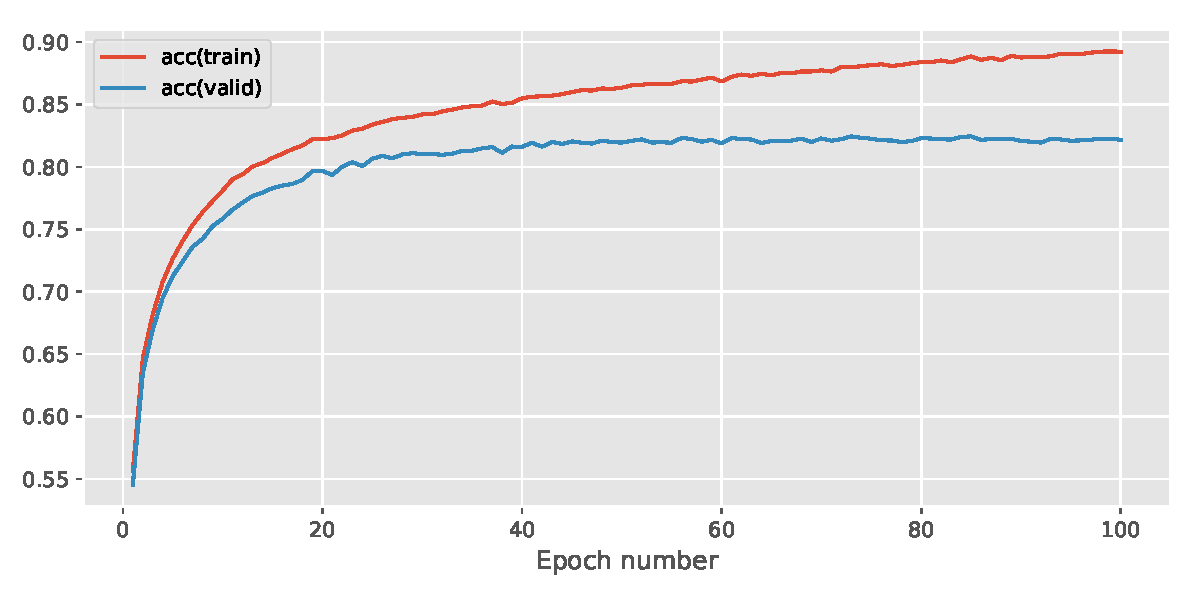
\includegraphics[width=0.45\textwidth]{./pic/q2/cw4_2_RMS_test_acc.pdf}}
	\subfigure[Adam for test set with the best learning rate]{
		\label{Fig.sub.2}
		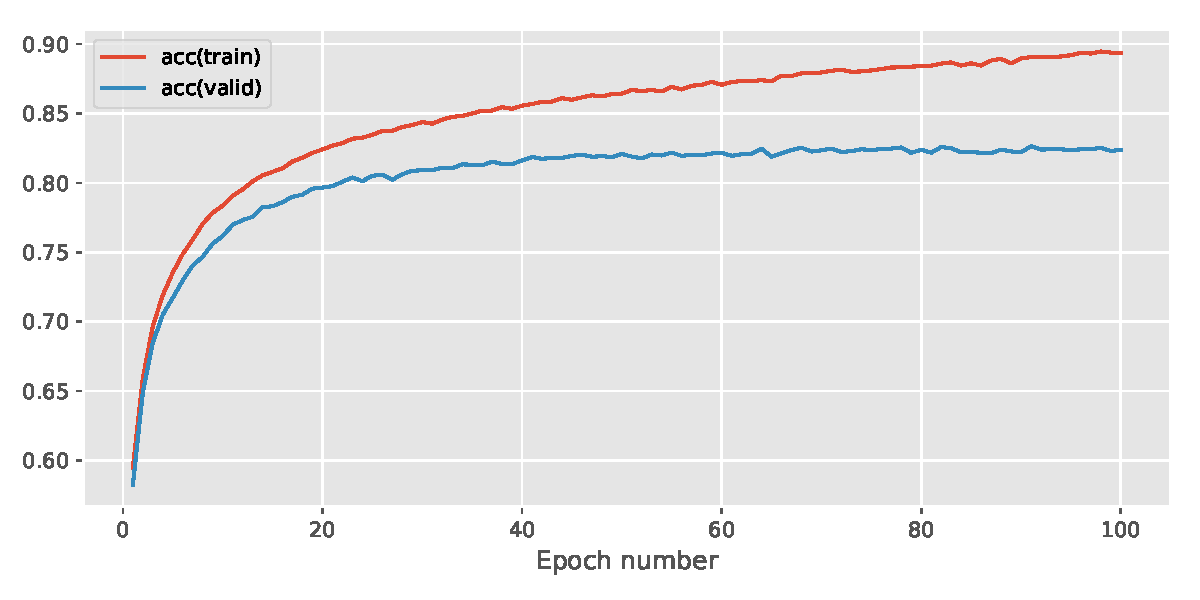
\includegraphics[width=0.45\textwidth]{./pic/q2/cw4_2_Adam_test_acc.pdf}}	
	\label{Fig.main}
\end{figure}

\begin{figure}[H]\label{q2:sgd}
	\centering  %图片全局居中
	\subfigure[SGD for test set with the best learning rate]{
		\label{Fig.sub.1}
		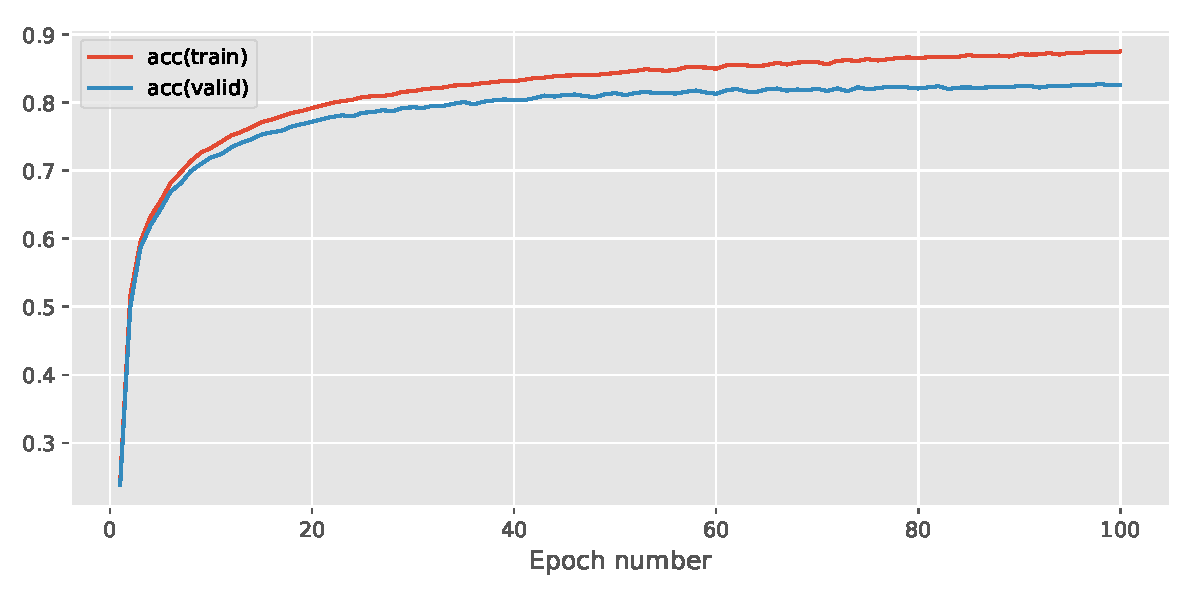
\includegraphics[width=0.45\textwidth]{./pic/q1/cw4_1_SGD_test_3Hidden_acc.pdf}}
	\label{Fig.main}
\end{figure}

% Table generated by Excel2LaTeX from sheet 'question2'
\begin{table}[htbp]
  \centering
  \caption{accuracy for test set}\label{q2:test}
    \begin{tabular}{|c|c|}
    \toprule
    \multirow{2}[2]{*}{algorithm} & \multirow{2}[2]{*}{accuracy(test)} \\
          &  \\
    \midrule
    \multicolumn{1}{|c|}{\multirow{2}[2]{*}{RMSProp}} & \multirow{2}[2]{*}{8.22E-01} \\
          &  \\
    \midrule
    \multicolumn{1}{|c|}{\multirow{2}[2]{*}{Adam}} & \multirow{2}[2]{*}{8.24E-01} \\
          &  \\
    \midrule
    \multicolumn{1}{|c|}{\multirow{2}[2]{*}{SGD}} & \multirow{2}[2]{*}{8.26E-01} \\
          &  \\
    \bottomrule
    \end{tabular}%
  \label{tab:addlabel}%
\end{table}%

According to the table\ref{q2:test}, SGD has a slight advantage in accuracy compared to the other two, but from the figure\ref{q2:rmspandadam}and the figure\ref{q2:sgd} RMSProp and Adam are faster than SGD in terms of fitting speed, and Adam is the fastest.


\section{Cosine annealing learning rate scheduler}

In this section, I will first introduce the cosine annealing scheduler and explain how it works. Then I will adjust the super parameters, train the system I think is the best, and then compare the performance of SGD and Adam in "no scheduler", "scheduler with no restarts", "special restarts" through test data.

\subsection{Algorithm}

cosine annealing scheduler update learning equation:

\begin{equation}\label{q3:cosine}
\eta_{t\;}=\;\eta_{min}^{(i)}+0.5(\eta_{max}^{(i)}\;-\;\eta_{min}^{(i)})(i\;+\;\cos(\frac{{\mathrm{\uppi T}}_\mathrm{cur}}{T_i}))
\end{equation}

In deep learning optimization, an important hyperparameter is the learning rate $\eta$. A good learning rate allows the neural network to achieve better fitting and faster fitting.

The cosine annealing scheduler is an algorithm that optimizes the learning rate. It can help the neural network adjust the learning rate. We can know by equation\ref{q3:consine} that we give a range of learning rate, the number of iterations of the cycle, and then the scheduler initializes the learning rate to a certain value and then gradually reduces it each time it restarts. . The key is to adjust the learning rate through a positive cosine annealing scheme, which will quickly reduce the learning rate.

\subsection{Experiment}

Training:Because in the section, we just compare SGD and Adam with using cosine annealing with no restarts, and with cosine annealing with restarts specified by an initial $T_i$ = 25 and $T_{mult}$ = 3.  "no restart" means the $T_i$ is equal to the epoch number(100), and $T_{mult}$ could be any number(I assign 1).So according to the equation\ref{q3:cosine},I only need to adjust the values of $\eta_{max}$  and $\eta_{min}$ to get the best performance of the neural network.I introduced a variable range to control the range of learning rates. The specific formula is as follows:
\begin{equation}
\begin{array}{l}\eta_{max\;=\;best\_learning\_rate\;\ast\;range}\\\eta_{min\;=\;best\_learning\_rate\;/\;range}\\\end{array}
\end{equation}

The best learning rates I have trained for SGD and Adam are 7.5e-3\ref{q1:test} and 1e-4\ref{q2:bestlearningrate} respectively.

for SGD:
\begin{figure}[H]\label{q3:sgdnorestart}
	\centering  %图片全局居中
	\subfigure[SGD with scheduler no restarts]{
		\label{Fig.sub.1}
		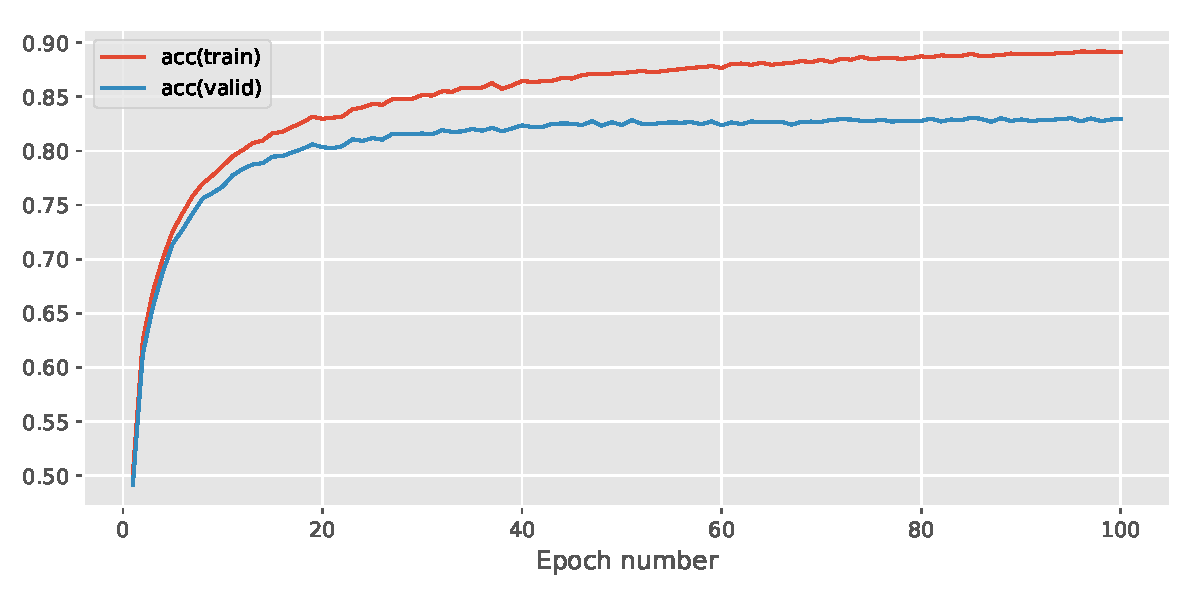
\includegraphics[width=0.45\textwidth]{./pic/q3/cw4_3_SGD_no_restart_acc.pdf}}
	\subfigure[SGD with scheduler special restarts]{
		\label{Fig.sub.2}
		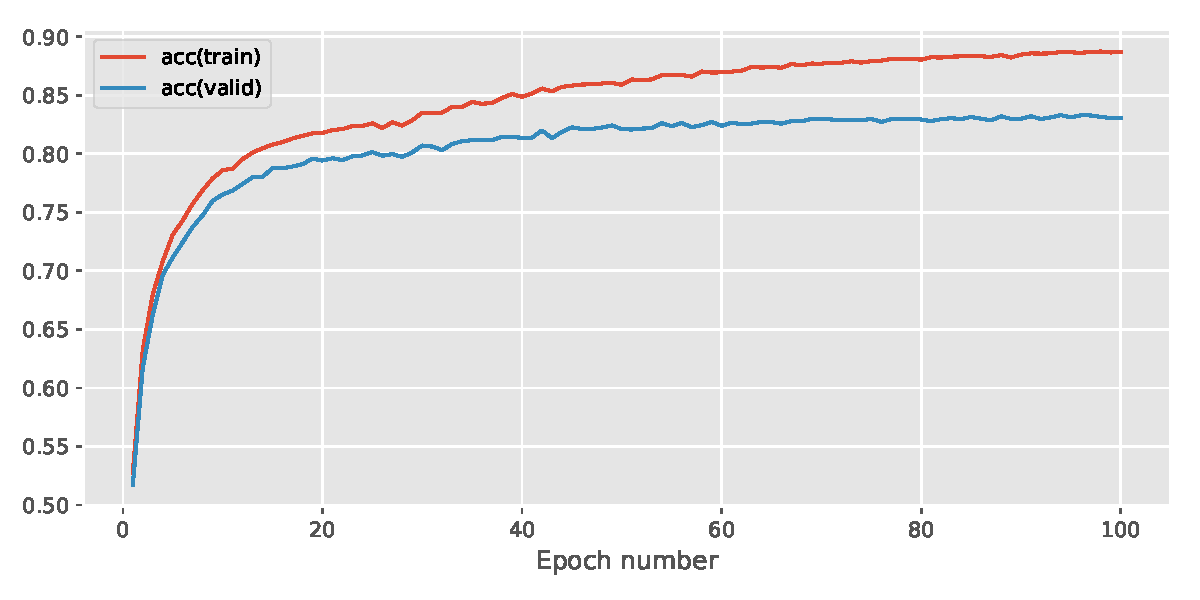
\includegraphics[width=0.45\textwidth]{./pic/q3/cw4_3_SGD_special_restart_acc.pdf}}	
	\label{Fig.main}
\end{figure}




for SGD:
\begin{figure}[H]\label{q3:sgdnorestart}
	\centering  %图片全局居中
	\subfigure[Adam with scheduler no restarts]{
		\label{Fig.sub.1}
		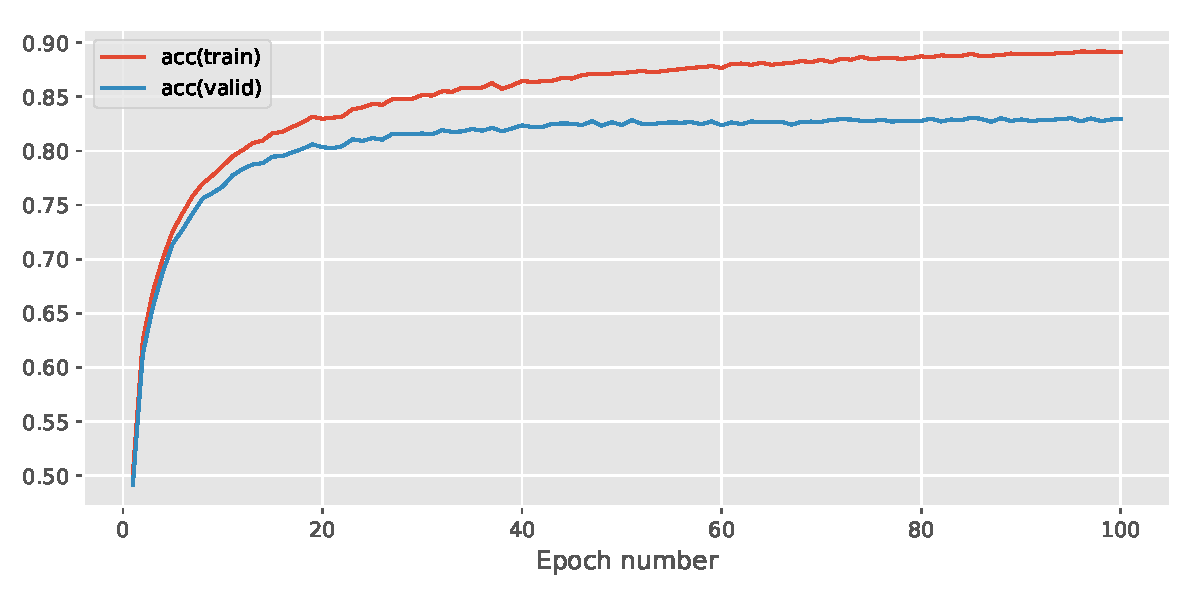
\includegraphics[width=0.45\textwidth]{./pic/q3/cw4_3_SGD_no_restart_acc.pdf}}
	\subfigure[Adam with scheduler special restarts]{
		\label{Fig.sub.2}
		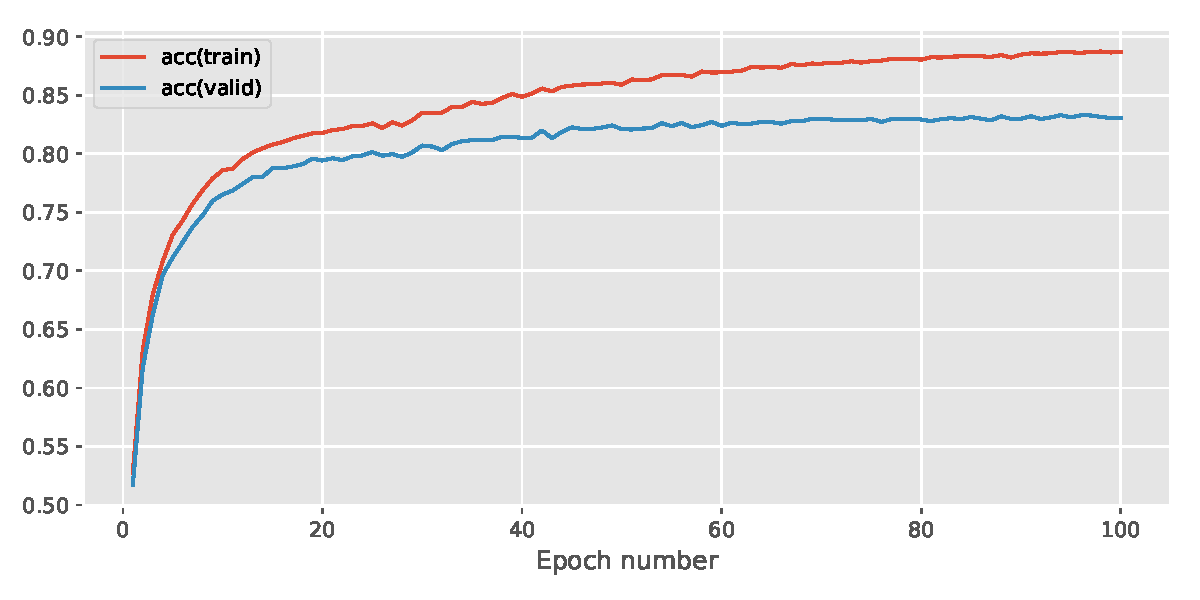
\includegraphics[width=0.45\textwidth]{./pic/q3/cw4_3_SGD_special_restart_acc.pdf}}	
	\label{Fig.main}
\end{figure}

From the figure, the accuracy of SGD With scheduler is not much improved, basically the same as before, but the fitting speed of SGD has improved a lot.

for Adam:
\begin{figure}[H]\label{q3:adamspecialRestart}
	\centering  %图片全局居中
	\subfigure[RMSProp for test set with the best learning rate]{
		\label{Fig.sub.1}
		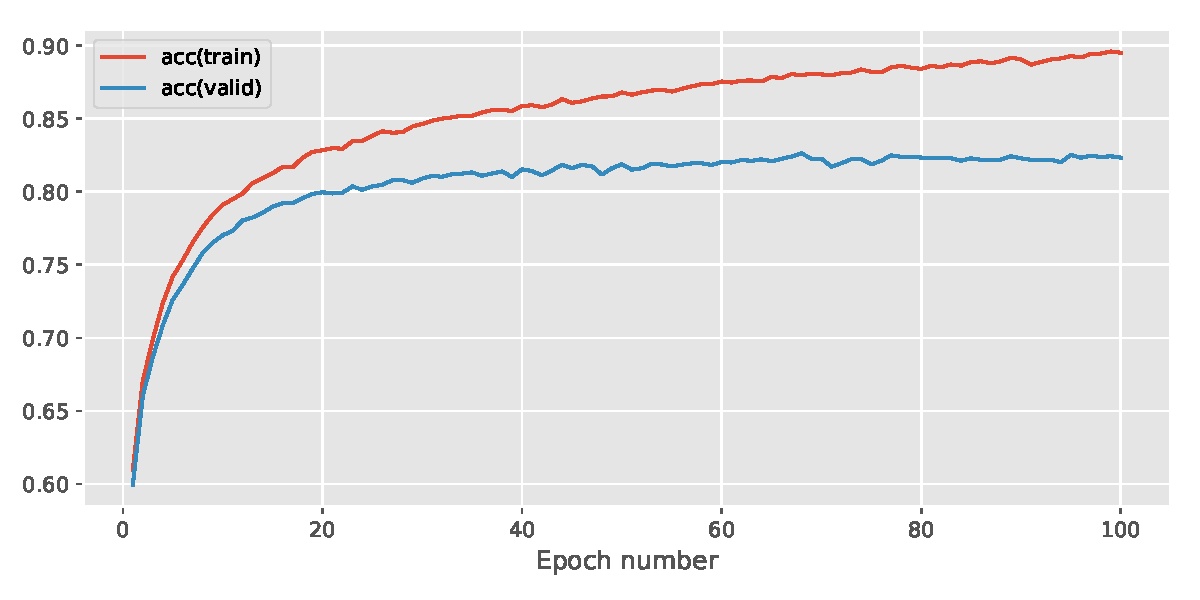
\includegraphics[width=0.45\textwidth]{./pic/q3/cw4_3_adam_no_restart__acc.pdf}}
	\subfigure[Adam for test set with the best learning rate]{
		\label{Fig.sub.2}
		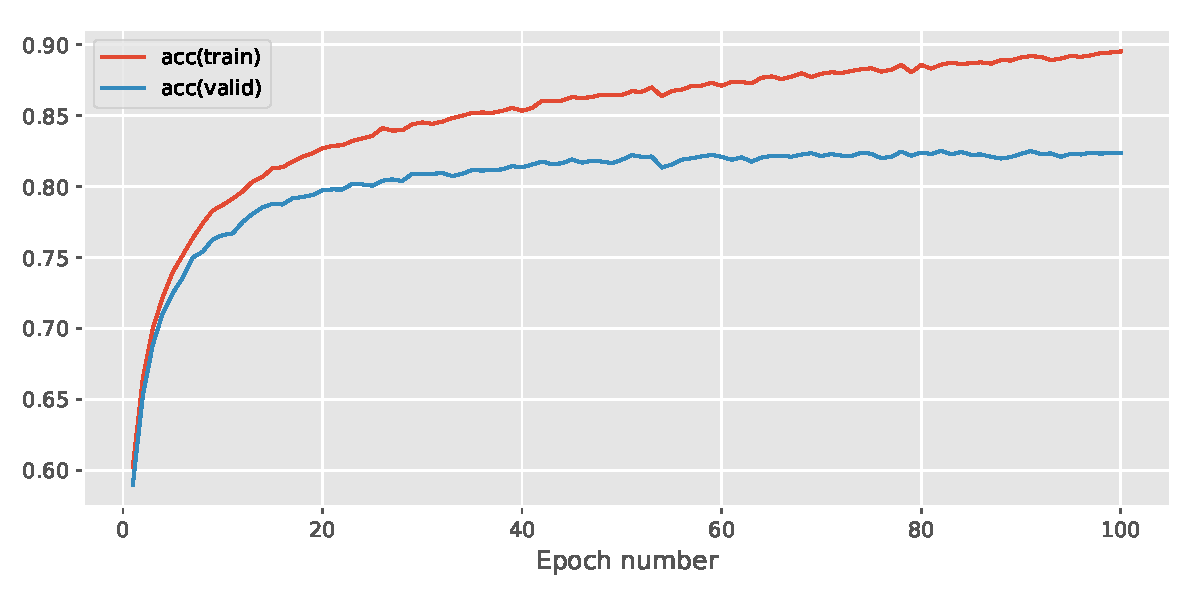
\includegraphics[width=0.45\textwidth]{./pic/q3/cw4_3_adam_special_restart__acc.pdf}}	
	\label{Fig.main}
\end{figure}

 


% Table generated by Excel2LaTeX from sheet 'quesiton3'
\begin{table}[htbp]\label{q3:sgdScheduler}
  \centering
  \caption{SGD for scheduler}
    \begin{tabular}{rrr}
    \multicolumn{1}{l}{range} & \multicolumn{1}{l}{no restart (acc(valid))} & \multicolumn{1}{l}{special restart(acc(valid))} \\
    1.05  & 8.36E-01 & 8.36E-01 \\
    1.1   & 8.38E-01 & 8.36E-01 \\
    1.15  & 8.39E-01 & 8.38E-01 \\
    1.2   & 8.40E-01 & 8.36E-01 \\
    2     & 8.40E-01 & 8.42E-01 \\
    3     & 8.38E-01 & 8.41E-01 \\
    5     & 8.37E-01 & 8.43E-01 \\
    10    & 8.32E-01 & 8.38E-01 \\
    \end{tabular}%
  \label{tab:addlabel}%
\end{table}%


% Table generated by Excel2LaTeX from sheet 'quesiton3'
\begin{table}[htbp]\label{q3:adamScheduler}
  \centering
  \caption{Adam for scheduler}
    \begin{tabular}{rrr}
    \multicolumn{1}{l}{range} & \multicolumn{1}{l}{no restart (acc(valid))} & \multicolumn{1}{l}{special restart(acc(valid))} \\
    1.05  & 8.39E-01 & 8.40E-01 \\
    1.1   & 8.36E-01 & 8.35E-01 \\
    1.15  & 8.36E-01 & 8.34E-01 \\
    1.2   & 8.37E-01 & 8.36E-01 \\
    2     & 8.36E-01 & 8.37E-01 \\
    3     & 8.34E-01 & 8.39E-01 \\
    5     & 8.28E-01 & 8.32E-01 \\
    10    & 8.23E-01 & 8.23E-01 \\
    \end{tabular}%
  \label{tab:addlabel}%
\end{table}%


According to table5 and table6, we can find the best range of learning for SGD\ref{q3:sgdScheduler} and Adam\ref{q3:adamScheduler} are 2 and 1.05 respectively.


Test:using test set to test the best SGD with no restarts and special restarts, comparing the no scheduler, the same for Adam.




\section{Regularization and weight decay with Adam}

\subsection{the problem using L2 regularization with Adam}

This is the equation of L2:
\begin{equation}
f^{reg}(x_t)\;=\;f_t(x_t)\;+\;\frac w2\vert\vert x\vert\vert_2^2
\end{equation}

L2 regularization means add L2 norm to loss function.According to the equation of Adam\ref{adam}, This means that the larger the value of $ g_t$, the larger the $v_t$ will be. When the weight is updated, an error will occur. The greater the weight, the smaller the penalty will be.


\subsection{solution}

Weight Decay is the solution.This algorithm adds an item when Adam updates the weights.

\begin{equation}
\begin{array}{l}\begin{array}{l}x_t\leftarrow\end{array}x_{t-1}\;-\eta\;\left(\frac{\alpha{\widehat m}_t}{\sqrt{{\widehat v}_t}+\in}\right)\end{array}\;+\:wx_{t-1}
\end{equation}

Weight decay is updated with the same coefficients for all weights. The larger the weight, the greater the penalty.


\subsection{Experiment}


\textbf{L2 VS Weight decay:}


\begin{figure}[H]\label{q4:adam}
	\centering  %图片全局居中
	\subfigure[L2]{
		\label{Fig.sub.1}
		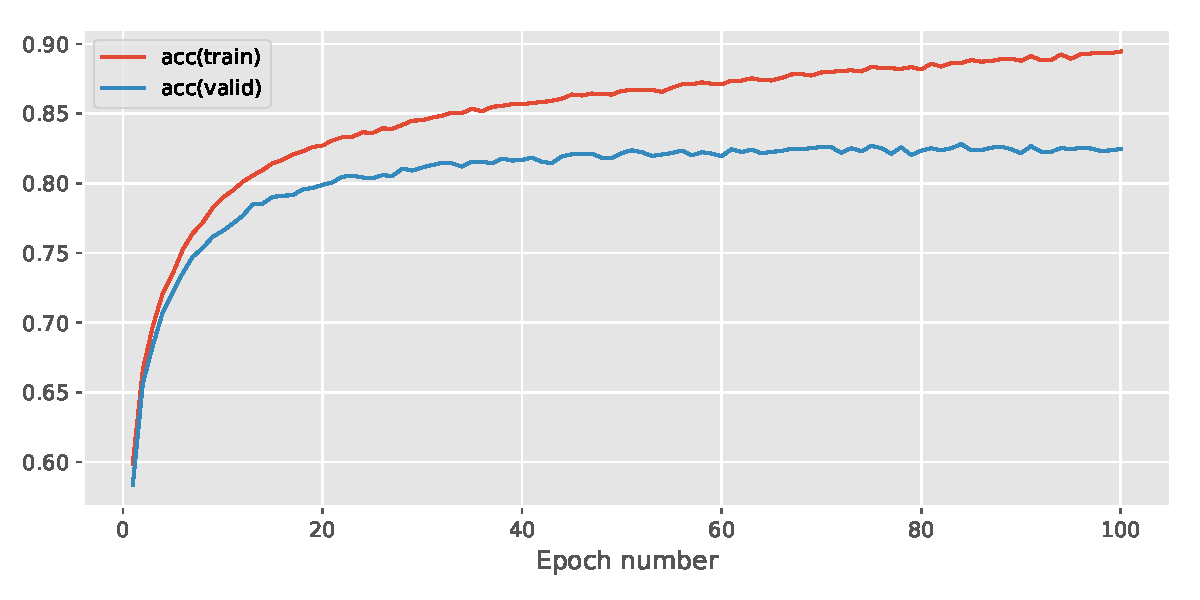
\includegraphics[width=0.45\textwidth]{./pic/q4/cw4_4_L2_acc.pdf}}
	\subfigure[Weight decay]{
		\label{Fig.sub.2}
		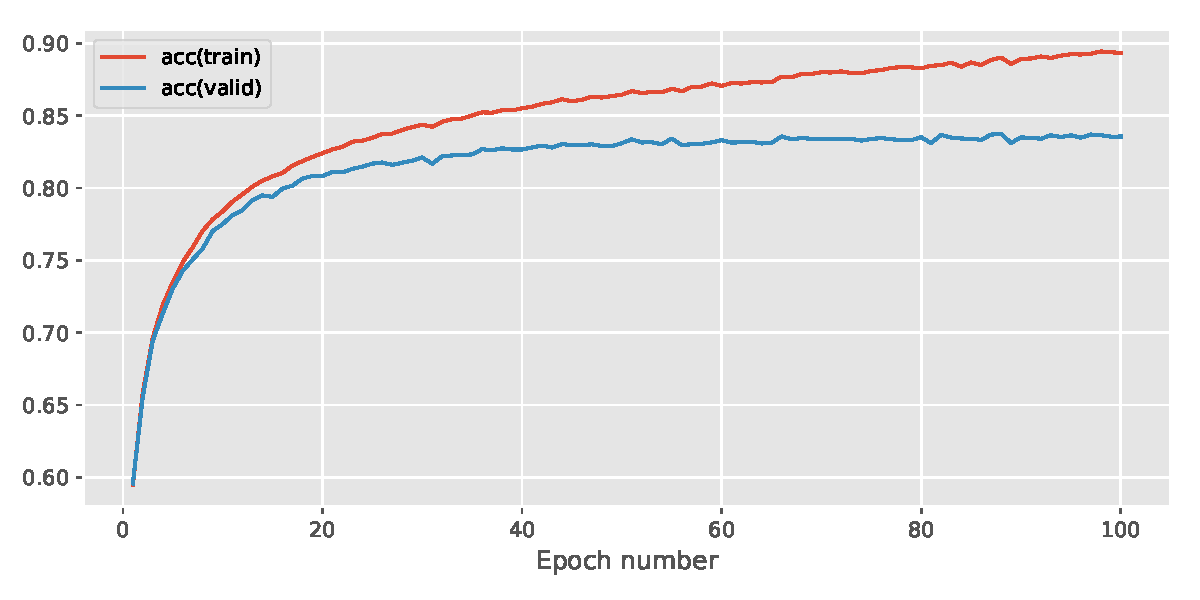
\includegraphics[width=0.45\textwidth]{./pic/q4/cw4_4_weight_decay_acc.pdf}}	
	\label{Fig.main}
\end{figure}

the accuracy of L2 is 0.825 and the data of Weight decay is 0.836,this also shows that weight decay is more suitable for Adam than L2.

\textbf{constant learning rate vs. cosine annealing schedule:}

constant learning rate\ref{q4:adam}


\textbf{no restarts in the scheduler vs. use of a warm restart:}




\section{Conclusions}
\label{sec:concl}

In conclusion, Although the fitting speed of SGD is not fast, its accuracy rate is not lower than RMSPorp and Adam. In the third part, after using scheduler with SGD, the fitting speed of SGD is obviously faster than before.
The Adam algorithm's fitting speed is very fast, but there is no obvious difference between the accuracy and the SGD. Later, the weight decay optimization is used to prevent the Adam from overfitting. The warm restarts can further accelerate the convergence speed of Adam, and can also improve Adam's convergence. Accuracy
The scheduler can help us get rid of the pain of debugging learning rate, although the accuracy of neural network learning by scheduler may not be the highest, but it can save a lot of time and indirectly improve efficiency.
The best systems is AdamW with restarts.


\bibliography{example-refs}

\end{document} 

